\subsection{COMPLETE GROUPS}

DEFINITION 2. A topological group is said to be complete if its left and right uniformities are structures of complete spaces.

From Proposition 2 of no. 1, for a group to be complete it is sufficient that one of its uniformities is a structure of a complete space. G is complete if and only if its associated Hausdorff group (§ 2, no. 6) is complete.

Every closed subgroup of a complete group is complete (Chapter II, § 3, no. 4, Proposition 8). Every product of complete groups is complete (Chapter II, § 3, no. 5, Proposition 10).

\pandocbounded{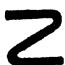
\includegraphics[keepaspectratio]{images/part002_8d186292.jpg}}

On the other hand, if G is a complete group and H is a closed normal subgroup of G, then the quotient group G/H is not necessarily complete (however, see Chapter IX, § 3, no. 1, Proposition 4).

PROPOSITION 4. If, in a topological group G, there is a neighbourhood V of e which is complete with respect to either the right or the left uniformity, then G is complete.

Suppose for example that V is complete with respect to the right uniformity, and let F be a Cauchy filter on \(G_{d}\) ; then F contains a \(V_{d}\) -small set M, and if \(x_{1} \in M\) we therefore have \(M \subset Vx_{1}\) . Hence the trace of F on the complete subspace \(Vx_{1}\) of \(G_{d}\) is a Cauchy filter, which converges to a point \(x_{0}\) ; since \(x_{0}\) is a cluster point of F, it is a limit of F (Chapter II, § 3, no. 2, Corollary 2 to Proposition 5).

COROLLARY 1. A locally compact group is complete.

For every compact space is complete with respect to its unique uniformity (Chapter II, § 4, no. 1, Theorem 1).

COROLLARY 2. Every locally compact subgroup of a Hausdorff topological group G is closed in G.

For every complete subspace of a Hausdorff uniform space is closed (Chapter II, § 3, no. 4, Proposition 8).

PROPOSITION 5. Let \(G_{1}\) be a topological group, let \(G_{2}\) be a complete Hausdorff topological group, and let \(H_{1}\) (resp. \(H_{2}\) ) be a dense subgroup of \(G_{1}\) (resp. \(G_{2}\) ). Then every continuous homomorphism u of \(H_{1}\) into \(H_{2}\) can be uniquely extended to a continuous homomorphism \(\overline{u}\) of \(G_{1}\) into \(G_{2}\) . Furthermore, if \(G_{1}\) is Hausdorff and complete, and if u is an isomorphism of \(H_{1}\) onto \(H_{2}\) , then \(\overline{u}\) is an isomorphism of \(G_{1}\) onto \(G_{2}\) .

\(\overline{u}\) is uniformly continuous with respect to the right uniformities of \(\mathbf{H}_1\) and \(\mathbf{H}_2\) (no. 1, Proposition 3), hence admits a unique extension to a mapping \(\overline{u}\) of \(\mathbf{G}_1\) into \(\mathbf{G}_2\) which is uniformly continuous with respect to the right uniformities of these groups (Chapter II, § 3, no. 6, Theorem 2). Moreover, by virtue of the principle of extension of identities (Chapter I, § 8, no. 1, Corollary 1 to Proposition 2), \(\overline{u}\) is a homomorphism of \(\mathbf{G}_1\) into \(\mathbf{G}_2\) , whence the first assertion of the Proposition. To prove the second assertion, it is enough to consider the isomorphism \(v\) of \(\mathbf{H}_2\) onto \(\mathbf{H}_1\) , which is the inverse of \(u\) , and its extension \(\overline{v}\) to a continuous homomorphism of \(\mathbf{G}_2\) into \(\mathbf{G}_1\) ; by reason of the uniqueness of the extension, \(\overline{v} \circ \overline{u}\) and \(\overline{u} \circ \overline{v}\) are the identity mappings of \(\mathbf{G}_1\) and \(\mathbf{G}_2\) respectively, and therefore (Set Theory, R, § 2, no. 12) \(\overline{u}\) is bijective.

\pandocbounded{
\includegraphics[keepaspectratio]{images/part002_2e6b534c.jpg}}

Remark. If the continuous homomorphism \(u\) is bijective, it does not follow in general that \(\overline{u}\) is either injective or surjective (cf.~Exercise 12); but see no. 5, Proposition 9.

